%!TEX root = ./Structure_rapport_final.tex

\renewcommand\thefigure{\thesection.\arabic{figure}}
\setcounter{figure}{0}

\section{Phylogenetic tree}
% Phylotree used in MM
\begin{figure} [!htbp]
	\begin{center}
		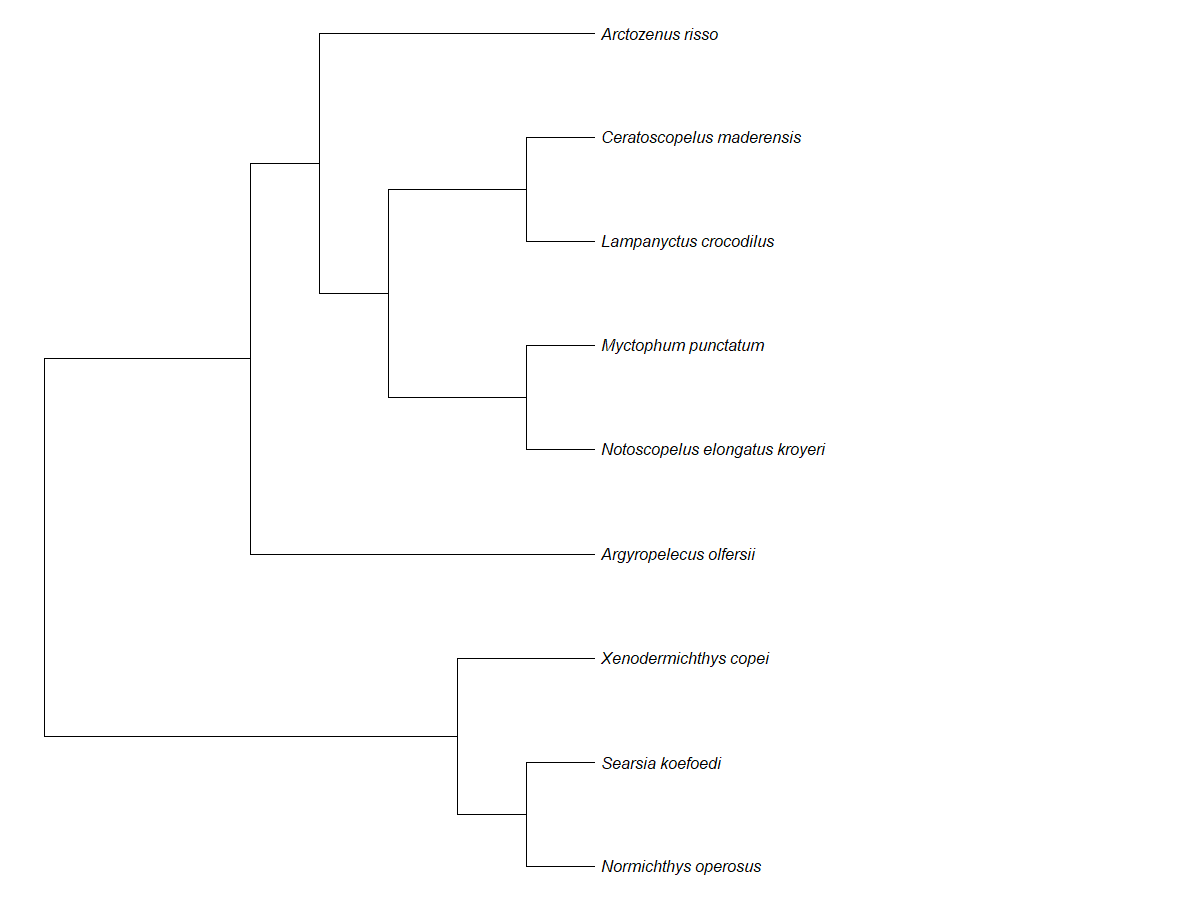
\includegraphics[width=0.8\textwidth]{phylogenic_tree.png}
	\end{center}
	\caption[Petite légende]{Phylogenic tree of studied species, using R \emph{rotl} package~\citep{opentreeoflife2019}~.}
	\label{fig:phylotree}
\end{figure}


\section{Morphological measurements}
%First figure: full body
\begin{figure} [!htbp]
	\begin{center}
		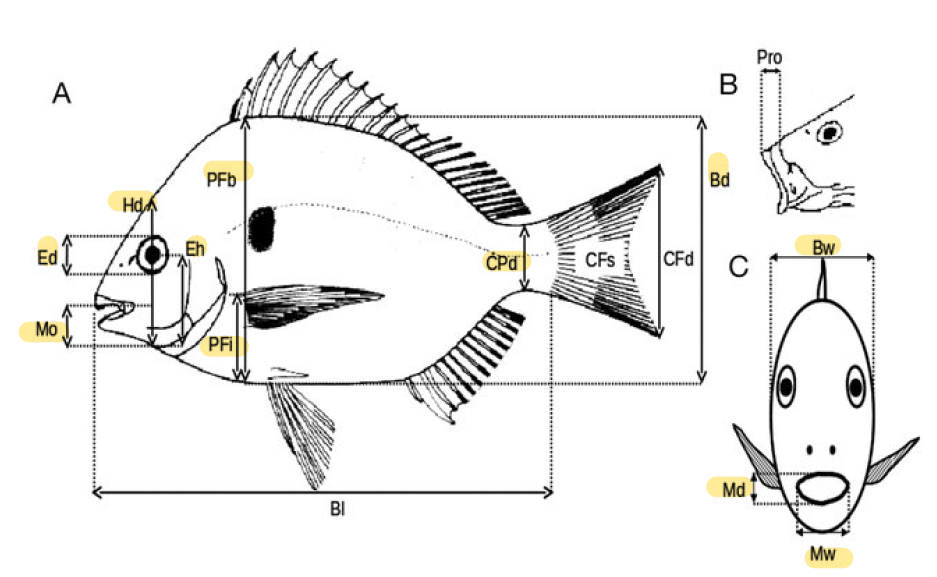
\includegraphics[width=0.8\textwidth]{Tp_Jerome_figure_1.png}
		\caption[Petite légende]{Morphological measurements, from \citet{albouy2011}. \textsc{bd}, body depth; \textsc{bw}, body width;\textsc{cpd}, caudal peduncle minimal depth; \textsc{ed}, eye diameter; \textsc{eh}, distance between the bottom of the head and the eye center along the head depth axis; \textsc{hd}, head depth along the vertical axis of the eye; \textsc{md}, mouth depth; \textsc{mo}, distance between the tip of the upper jaw and bottom of the head; \textsc{mw}, mouth width; \textsc{pfb}, body depth at the level of the pectoral insertion; \textsc{pfi}, distance between the insertion of pectoral fin and the bottom of the body.}
	\label{fig:full_body}
	\end{center}
\end{figure}


%Second figure: zoom on the head
\begin{figure} [!htbp]
	\begin{center}
		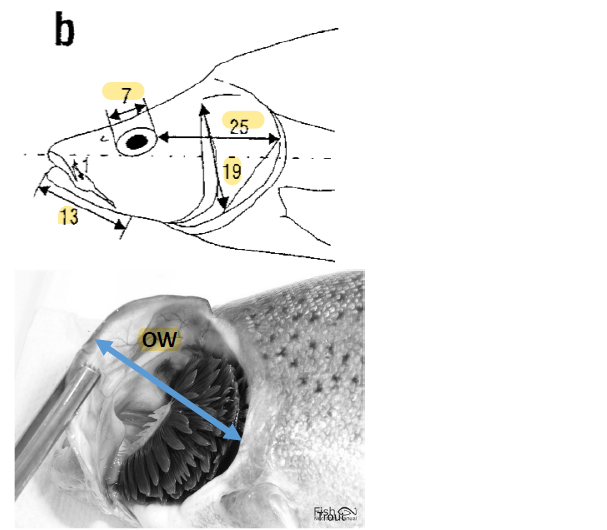
\includegraphics[width=0.8\textwidth]{Tp_Jerome_figure_2.png}
		\caption[Petite légende]{Morphological measurements of the head, from \citet{diderich2006}, following \citet{sibbing2000}. 7 being \textsc{ed}, eye diameter; 13 \textsc{ljl}, distance between the tip and the insertion point of lower jaw; 19 \textsc{od}, depth of the operculum from point of insertion to bottom; 25 \textsc{pol}, shortest distance between the eye and the end of the head; \textsc{ow}, operculum maximum width.}
	\label{fig:head}
	\end{center}
	
\end{figure}


%Third figure: fin length
\begin{figure} [!htbp]
	\begin{center}
		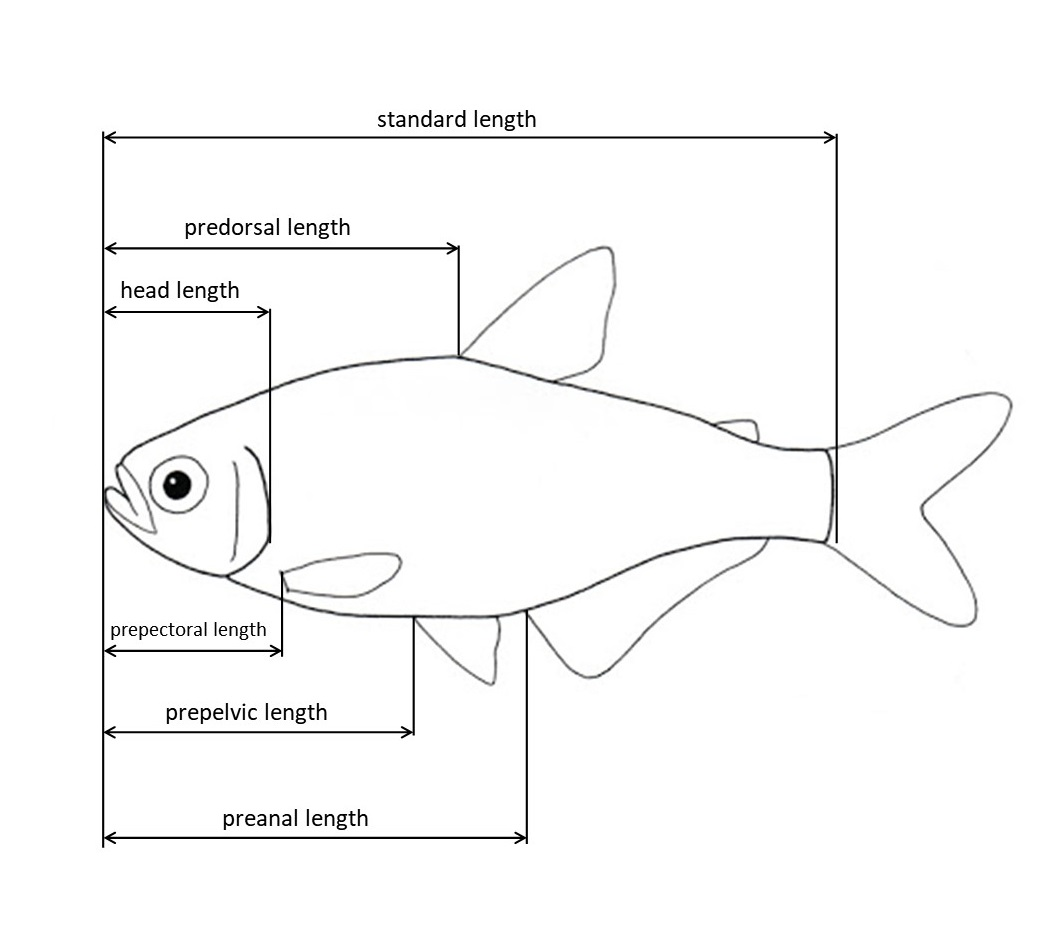
\includegraphics[width=0.8\textwidth]{Figure_3.jpg}
		\caption[Petite légende]{Morphological measurements of the head, adpated from \citet{keat-chuanng2017,habib2019}. \textsc{hl}, head length, from the nose to the closest-to-caudal-fin point of the operculum; \textsc{pal}, distance bewteen the tip of the nose and the insertion of anal fin; \textsc{pdl}, distance bewteen the tip of the nose and the insertion of dorsal fin, \textsc{ppl}, distance bewteen the tip of the nose and the insertion of pectoral fin; \textsc{pvl}, distance bewteen the tip of the nose and the insertion of pelvic fin;  \textsc{sl}, standard length.}
		\label{fig:fin}
	\end{center}
	
\end{figure}


%Fourth and fifth figures: Git and OGA
\begin{figure} [!htbp]
	\begin{center}
	\begin{minipage}{0.45\textwidth}
		\centering
		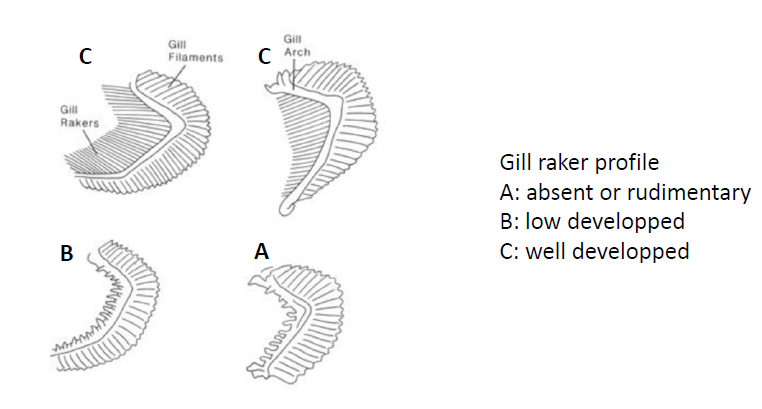
\includegraphics[width=1	\textwidth]{Tp_Jerome_figure_Git.png}
		\caption[Petite légende]{Scores of gill rakers types \textsc{git}, based on their length.}
		\label{fig:git}
	\end{minipage}\hfill
	\begin{minipage}{0.45\textwidth}
		\centering
		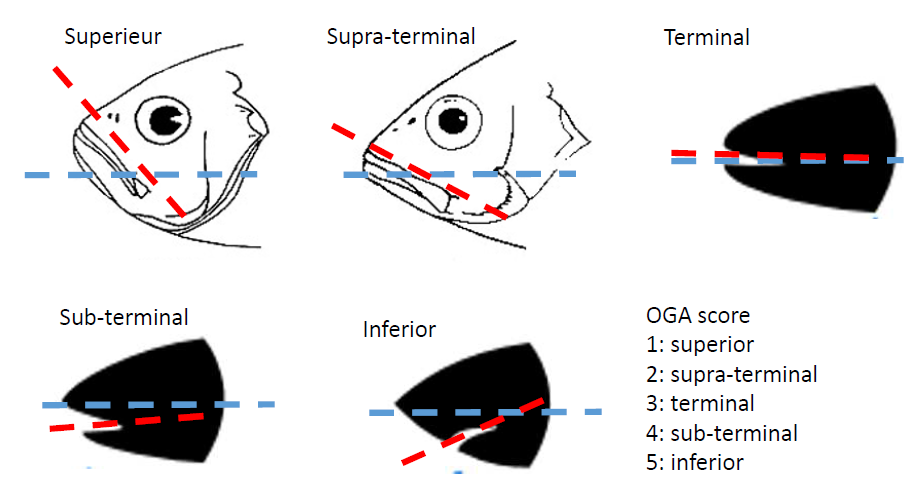
\includegraphics[width=1\textwidth]{Tp_Jerome_figure_Oga.png}
		\caption[Petite légende]{Scores of oral gape axis \textsc{oga}, based on the angle between mouth orientation (red) and a fictive mid-depth lateral lign (blue).}
		\label{fig:oga}
	\end{minipage}
	\end{center}
	
\end{figure}

\section{Correlation plot}
% Correlation circle to help understand FAMD results
\begin{figure} [!htbp]
	\begin{center}
		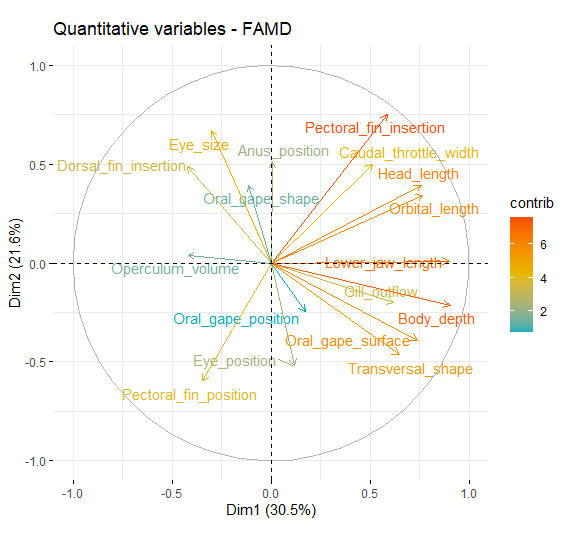
\includegraphics[width=0.8\textwidth]{Correlation_circle.png}
	\end{center}
	\caption{Correlation circle of axis 1 and 2. The 'contrib' variable refers to the representativity of the variable on the axis. The higher the value is, the more the corresponding variable contributes to the axis.}
	\label{fig:corr_circ_12}
\end{figure}

\begin{figure} [!htbp]
	\begin{center}
		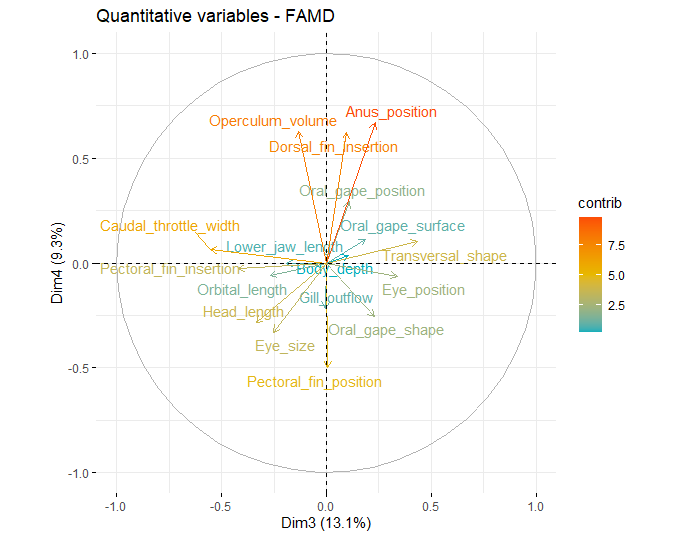
\includegraphics[width=0.8\textwidth]{coord_plot_34.png}
	\end{center}
	\caption{Correlation circle of axis 3 and 4. The 'contrib' variable refers to the representativity of the variable on the axis. The higher the value is, the more the corresponding variable contributes to the axis.}
	\label{fig:corr_circ_34}
\end{figure}

